\documentclass{article}

\usepackage[utf8]{inputenc}
\usepackage[brazil]{babel}

\title{Exercício 1: Gaussiana no Espaço $R^2$}
\author{Rúbia Reis Guerra \\ 2013031143}

\usepackage{Sweave}
\begin{document}
\Sconcordance{concordance:gaussr2.tex:gaussr2.Rnw:%
1 8 1 1 0 11 1 1 2 1 0 2 1 1 7 6 0 1 4 2 0 2 1 1 4 2 0 1 1 1 3 1 0 1 1 %
1 3 6 0 1 2 2 1 1 6 5 0 3 1 1 3 1 0 3 1 1 3 1 0 1 1 1 4 2 0 1 1 1 2 1 1 %
1 2 1 11 13 0 1 2 2 1 1 5 4 0 1 2 5 0 1 2 1 4 3 0 1 1 1 2 5 0 1 2 2 1 1 %
4 3 0 1 4 2 0 1 2 1 0 1 2 5 0 1 2 1 5 4 0 1 1 1 2 1 0 1 1 1 2 5 0 1 2 1 %
1}

\maketitle

\section{Gaussiana no Espaço $R^2$}
Os métodos Naive Bayes são um conjunto de algoritmos de aprendizagem supervisionada com base no teorema de Bayes, a partir da suposição "ingênua" de independência entre cada par de características. Nesta atividade, foi proposta a amostragem de dados de duas distribuições normais bivariadas com coefieciente de correlação nulo, seguida da avaliação de suas respectivas densidades de probabilidade e, enfim, da geração da superfície de separação das classes iniciais.

%##################################

\subsection{Implementação}
Inicialmente, são geradas duas distribuições de duas variáveis ($x$ e $y$), caracterizadas por $\mathcal{N}(2,2,\sigma^2)$ e $\mathcal{N}(4,4,\sigma^2)$ e coeficiente de correlação nulo:

\begin{Schunk}
\begin{Sinput}
> library('plot3D')
> library('MASS')
> rm(list=ls())
> ########################################
> # Funções #
> fnormal2var <- function(x,y,mx,my,sx,sy,cr){
+   (1/(2*pi*sx*sy*sqrt(1-cr*cr)))*
+     exp((-0.5*(1-cr*cr))*((((x-mx)^2)/(sx^2))+
+                             (((y-my)^2)/(sy^2))-
+                             (2*cr*((x-mx)*(y-my))/sy*sx)))}
> ########################################
> # Parâmetros iniciais #
> N <- 100
> minseq <- 0
> maxseq <- 6
> ########################################
> # Gerando dados amostrados das distribuições m1=(2,2)', m2=(4,4)' #
> c1 <- matrix(rnorm(N*2),ncol=2)*0.5+c(2,2)
> c2 <- matrix(rnorm(N*2),ncol=2)*0.5+c(4,4)
> plot(c1[,1], c1[,2], col='red', type='p', xlim=c(minseq,maxseq), 
+      ylim=c(minseq,maxseq),xlab='x',ylab='y')
> par(new=T)
> plot(c2[,1], c2[,2], col='blue', type='p', xlim=c(minseq,maxseq), 
+      ylim=c(minseq,maxseq),xlab='',ylab='',
+      sub='Figura 1: Dados amostrados das distribuições normais')
\end{Sinput}
\end{Schunk}
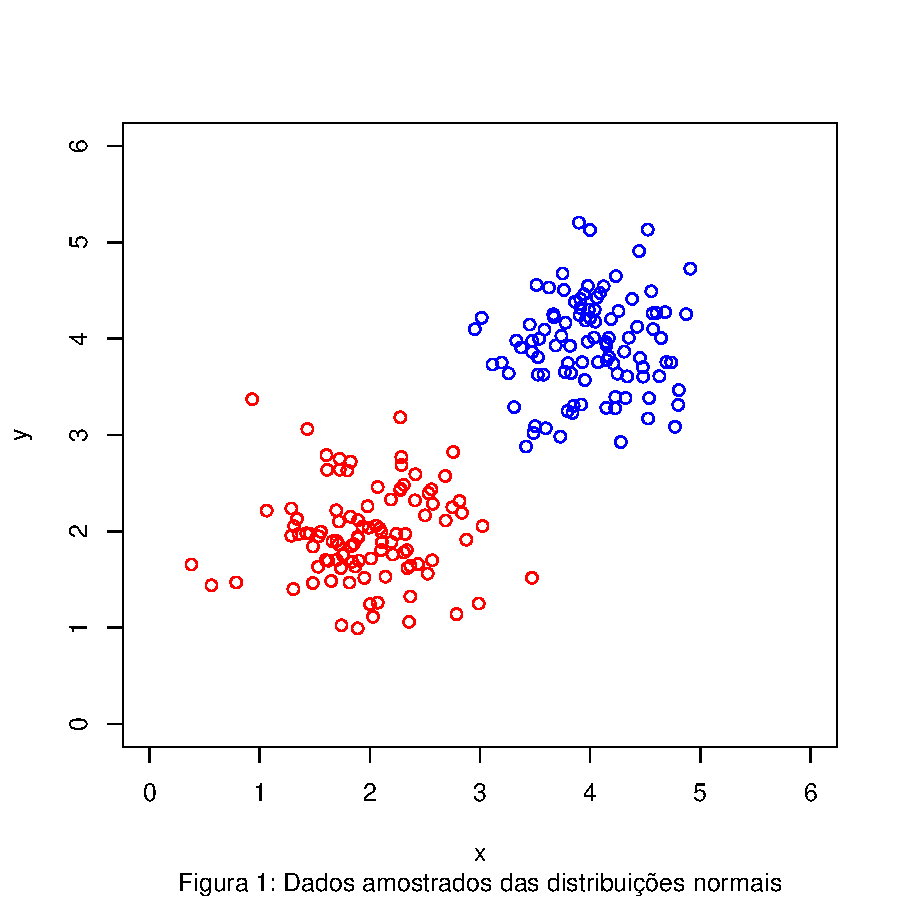
\includegraphics{gaussr2-001}

Em seguida, são estimados os parâmetros de cada uma das distribuições e suas respectivas densidades de probabilidade, utilizando a função \textit{fnormal2var}:

\begin{Schunk}
\begin{Sinput}
> ########################################
> # Estimando parâmetros das densidades #
> 
> # Médias
> m11 <- mean(c1[,1]) # C1
> m12 <- mean(c1[,2]) # C1
> m21 <- mean(c2[,1]) # C2
> m22 <- mean(c2[,2]) # C2
> # Desvios pradão
> s11 <- sd(c1[,1]) # C1
> s12 <- sd(c1[,2]) # C1
> s21 <- sd(c2[,1]) # C2
> s22 <- sd(c2[,2]) # C2
> # Coeficientes de correlação
> cr1 <- cor(c1[,1],c1[,2])
> cr2 <- cor(c2[,1],c2[,2])
> ########################################
> # Estimando a densidade de C1 e C2 #
> seqi <- seq(minseq,maxseq,0.1)
> seqj <- seq(minseq,maxseq,0.1)
> M1 <- matrix(0,nrow=length(seqi),ncol=length(seqj))
> M2 <- matrix(0,nrow=length(seqi),ncol=length(seqj))
> ci <- 0
> for (i in seqi)
+ {
+   cj <- 0
+   ci<- ci + 1
+   for (j in seqj)
+   {
+     cj <- cj + 1
+     M1[ci,cj]<-fnormal2var(i,j,m11,m12,s11,s12,cr1)
+     M2[ci,cj]<-fnormal2var(i,j,m21,m22,s21,s22,cr2)
+   }
+ }
\end{Sinput}
\end{Schunk}

Gráficos obtidos:

\begin{Schunk}
\begin{Sinput}
> ########################################
> # Gráficos das densidades de probabilidade #
> persp3D(seqi,seqj,M1,clim=c(0,0.8),colkey=T, 
+         sub='Figura 2: Densidades de probabilidade das distribuições')
> persp3D(seqi,seqj,M2,clim=c(0,0.8),add=T,colkey=T,
+         sub='')
\end{Sinput}
\end{Schunk}
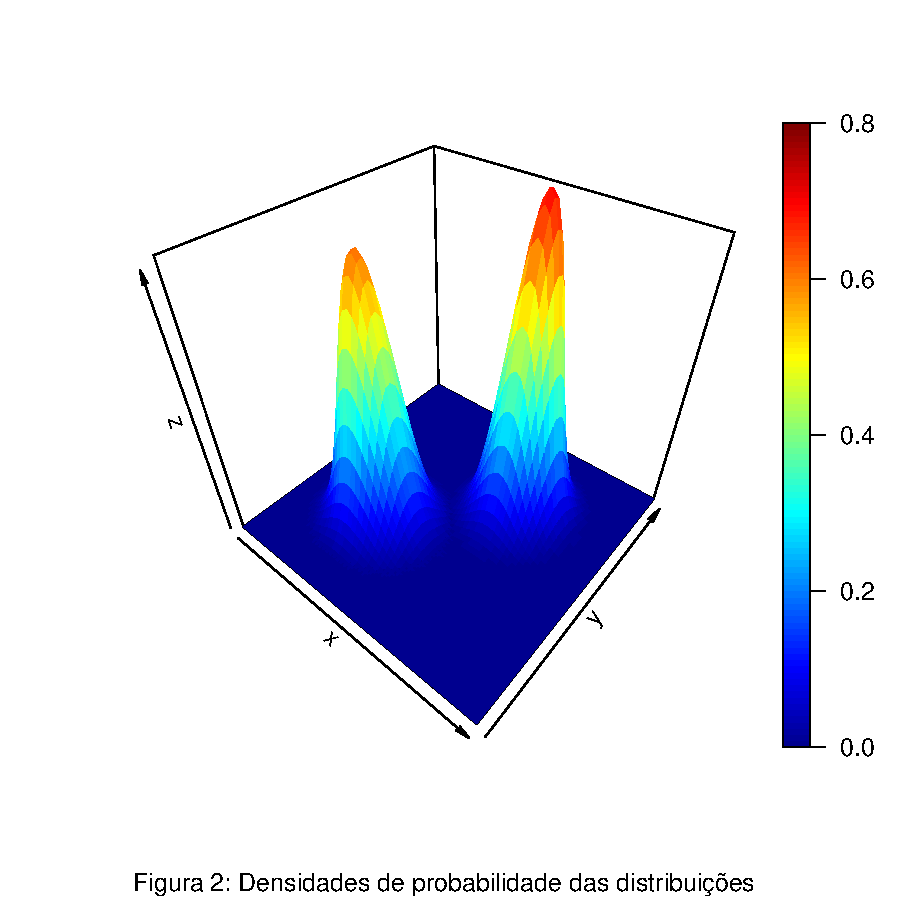
\includegraphics{gaussr2-003}

\begin{Schunk}
\begin{Sinput}
> ########################################
> # Curvas de nível da densidade de probabilidade #
> contour2D(M1,seqi,seqj)
> par(new=T)
> contour2D(M2, seqi,seqj,
+           sub='Figura 3: Curvas de nível das densidades de probabilidade')
\end{Sinput}
\end{Schunk}
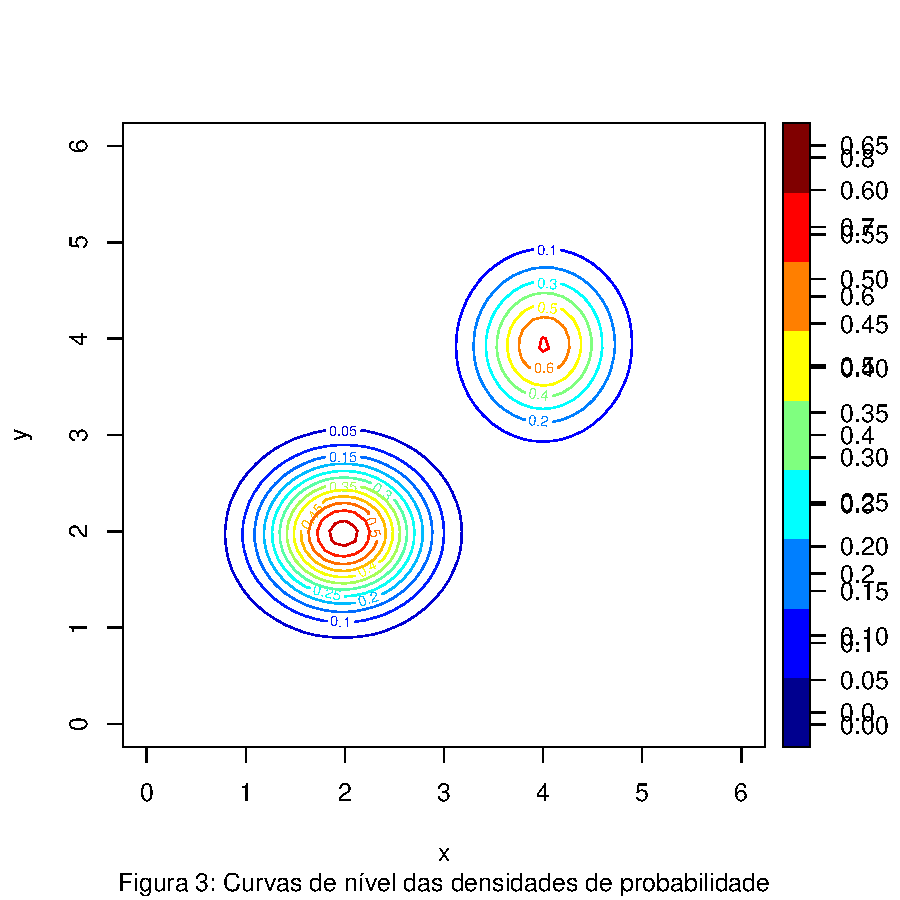
\includegraphics{gaussr2-004}

Enfim, é determinada a superfície de separação das distribuições:

\begin{Schunk}
\begin{Sinput}
> ########################################
> # Superfície de separação #
> classx<-0.7*(M1 >= M2)
> # Superfície de separação - 3D #
> persp3D(seqi,seqj,M1,clim=c(0,0.8),colkey=T,
+         sub='Figura 4: Superfície de separação - 3D')
> persp3D(seqi,seqj,M2,clim=c(0,0.8),add=T,colkey=T,
+         sub='')
> persp3D(seqi,seqj,classx,clim=c(1.5,0), zlim=c(0,2),add=T,colkey=F,
+         sub='')
\end{Sinput}
\end{Schunk}
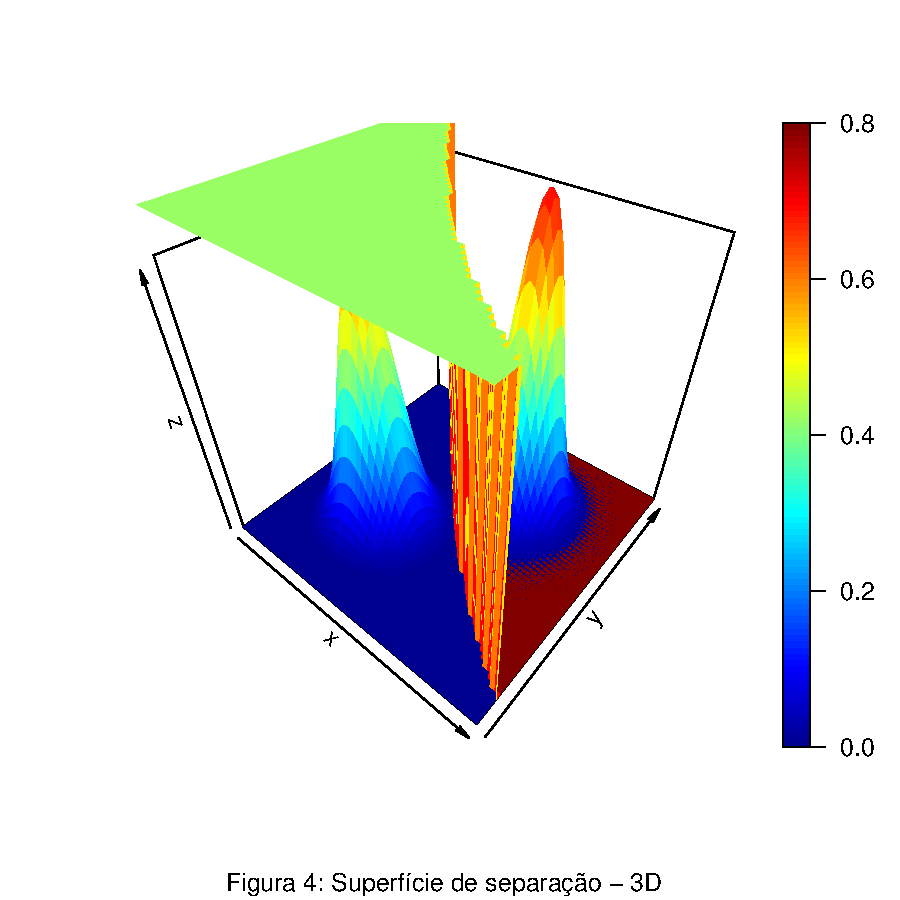
\includegraphics{gaussr2-005}

\begin{Schunk}
\begin{Sinput}
> ########################################
> # Superfície de separação - 2D #
> plot(c1[,1], c1[,2], col='red', type='p', xlim=c(minseq,maxseq), 
+      ylim=c(minseq,maxseq),xlab='x',ylab='y')
> par(new=T)
> plot(c2[,1], c2[,2], col='blue', type='p', xlim=c(minseq,maxseq), 
+      ylim=c(minseq,maxseq),xlab='',ylab='')
> par(new=T)
> contour2D(classx,seqi,seqj,col='black',
+            sub='Figura 5: Superfície de separação - 2D')
\end{Sinput}
\end{Schunk}
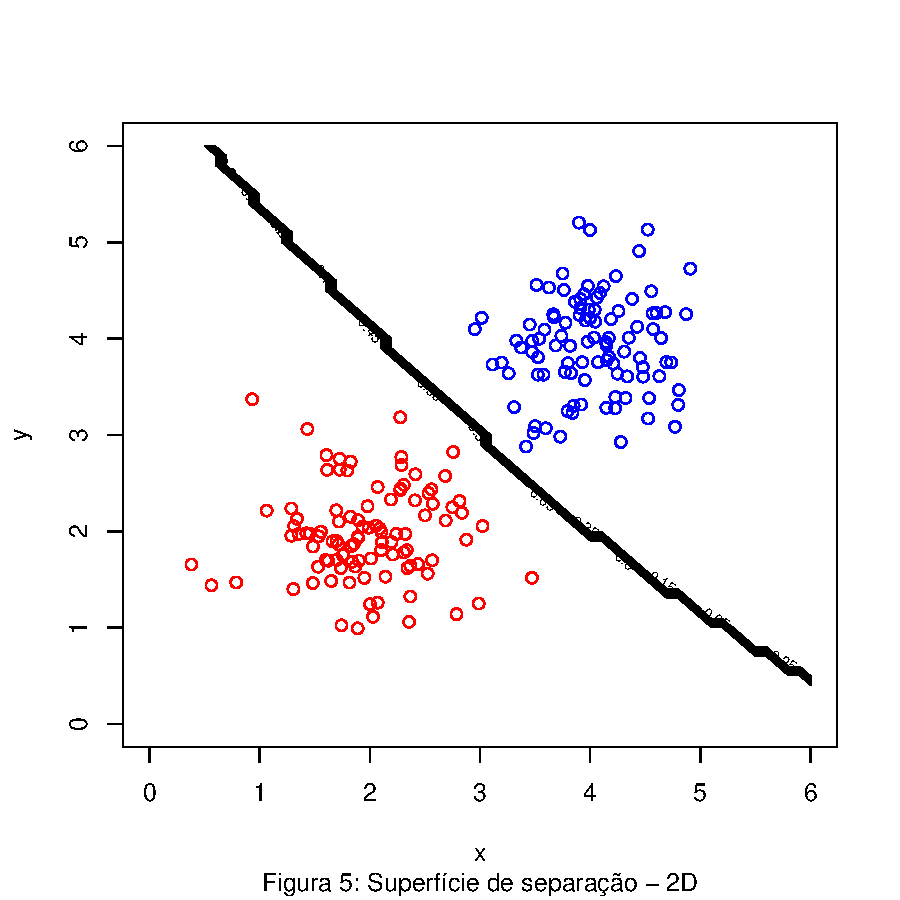
\includegraphics{gaussr2-006}

\end{document}
